\section{Анализ затрат на реализацию проекта}

\subsection{Анализ затрат на изготовление продукта}

После определения трудоёмкости работ, состава исполнителей и
календарного графика выполнения проекта необходимо выполнить расчёт
затрат на разработку программного продукта. Структура затрат должна
отражать основные ресурсы, необходимые для создания разрабатываемой
системы, и включать расходы на оплату труда исполнителей,
оборудование, амортизационные отчисления, расходные материалы,
организацию рабочих мест и накладные расходы.

Общая величина затрат на изготовление продукта определяется по
формуле:

\begin{equation}
C = C_{\text{з.п.}} + C_{\text{об}} + C_{\text{аморт}} +
C_{\text{расх}} + C_{\text{орг}} + C_{\text{накл}}.
\end{equation}

\subsubsection*{Затраты на заработную плату исполнителей}

Затраты на заработную плату определяются как сумма основной
заработной платы, дополнительной заработной платы и страховых
отчислений:

\begin{equation}
C_{\text{з.п.}} = C_{\text{осн}} + C_{\text{доп}} + C_{\text{отч}}.
\end{equation}

Дополнительная заработная плата составляет 20\% от основной:

\begin{equation}
C_{\text{доп}} = 0.2 \cdot C_{\text{осн}}.
\end{equation}

Страховые отчисления составляют 30\% от суммы основной и
дополнительной заработной платы:

\begin{equation}
C_{\text{отч}} = (C_{\text{осн}} + C_{\text{доп}})\cdot 0.3.
\end{equation}

Расчёт основной заработной платы выполняется на основе трудоёмкости
работ и месячных окладов исполнителей. Часовая тарифная ставка
определяется исходя из месячного фонда рабочего времени 168 часов:

\begin{equation}
C_{\text{час}} = \frac{C_{\text{мес}}}{168}.
\end{equation}

При расчёте фонда заработной платы необходимо учитывать не только
суммарную трудоёмкость проекта, равную 436 чел.-ч, но и фактическое
распределение работ между исполнителями. В рассматриваемом проекте
этапы анализа требований и подготовки документации выполняются
аналитиком, проектирование архитектуры и проработка взаимодействия
модулей --- архитектором, реализация библиотеки трассировки ---
старшим разработчиком, а разработка подсистем агрегации и обработки
трасс --- разработчиком. При этом этап тестирования и отладки
выполняется совместно разработчиком и старшим разработчиком, поэтому
его трудоёмкость учитывается в фонде рабочего времени обоих
исполнителей. В результате суммарные трудозатраты по исполнителям
составляют 480 чел.-ч, что превышает общую трудоёмкость проекта за
счёт параллельного участия двух специалистов в заключительном этапе.

Для расчёта примем следующие значения месячных окладов:
аналитик --- 120000 руб., архитектор --- 150000 руб., разработчик ---
140000 руб., старший разработчик --- 170000 руб.

\begin{table}[h]
\centering
\caption{Расчёт основной заработной платы исполнителей}
\label{tab:salary_calc}
\resizebox{\textwidth}{!}{
\begin{tabular}{|c|p{3.7cm}|c|c|c|c|c|}
\hline
№ & Должность & Оклад, руб. &
Часовая ставка, руб./ч &
Трудозатраты, ч &
Трудозатраты, дни &
Оплата труда, руб. \\ \hline

1 & Аналитик &
120000 & 714.29 &
116 & 14.5 &
82857.14 \\ \hline

2 & Архитектор &
150000 & 892.86 &
84 & 10.5 &
75000.00 \\ \hline

3 & Разработчик &
140000 & 833.33 &
124 & 15.5 &
103333.33 \\ \hline

4 & Старший разработчик &
170000 & 1011.90 &
156 & 19.5 &
157857.14 \\ \hline

\multicolumn{6}{|r|}{Итого основная заработная плата $C_{\text{осн}}$} &
419047.61 \\ \hline

\end{tabular}
}
\end{table}

Тогда дополнительная заработная плата составит:

\begin{equation}
C_{\text{доп}} = 0.2 \cdot 419047.61 = 83809.52 \text{ руб.}
\end{equation}

Страховые отчисления:

\begin{equation}
C_{\text{отч}} =
(419047.61 + 83809.52)\cdot 0.3 = 150857.14 \text{ руб.}
\end{equation}

Полные затраты на заработную плату исполнителей:

\begin{equation}
C_{\text{з.п.}} =
419047.61 + 83809.52 + 150857.14 = 653714.27 \text{ руб.}
\end{equation}

\subsubsection*{Затраты на оборудование}

Для реализации проекта требуется использование вычислительной техники,
необходимой для разработки, тестирования и выполнения программного
инструмента. В отличие от проектов, ориентированных на эксплуатацию в
крупной инфраструктуре, разрабатываемая система не требует выделенных
серверных мощностей и может быть реализована на персональных
компьютерах исполнителей.

Тем не менее, для обеспечения полноценного процесса разработки и
тестирования необходимо предусмотреть рабочие станции для участников
проекта, а также вспомогательное оборудование для хранения данных и
резервного копирования.

Состав необходимого оборудования и затраты на его приобретение
приведены в таблице~\ref{tab:equipment}.

\begin{table}[h]
\centering
\caption{Затраты на закупку оборудования и технических средств}
\label{tab:equipment}
\resizebox{\textwidth}{!}{
\begin{tabular}{|c|p{7cm}|c|c|c|}
\hline
№ & Наименование оборудования & Количество &
Цена за единицу, руб. & Сумма, руб. \\ \hline

1 & Ноутбук для разработки &
4 & 80000 & 320000 \\ \hline

2 & Рабочая станция старшего разработчика (повышенной производительности) &
1 & 120000 & 120000 \\ \hline

3 & Внешний накопитель для хранения и резервного копирования данных &
1 & 10000 & 10000 \\ \hline

4 & Источник бесперебойного питания &
1 & 15000 & 15000 \\ \hline

5 & Сетевое оборудование (маршрутизатор) &
1 & 8000 & 8000 \\ \hline

\multicolumn{4}{|r|}{Итого $C_{\text{об}}$:} & 473000 \\ \hline

\end{tabular}
}
\end{table}

Таким образом, затраты на закупку оборудования и технических средств
составляют:

\begin{equation}
C_{\text{об}} = 473000 \text{ руб.}
\end{equation}

\subsubsection*{Амортизационные расходы на оборудование}

Поскольку оборудование используется в проекте в течение ограниченного
периода времени, необходимо определить амортизационные расходы за
время выполнения работ.

Амортизационные расходы рассчитываются по формуле:

\begin{equation}
C_{\text{аморт}} =
\sum_i \frac{C_{\text{об}i} \cdot \Delta t_i}{D_{\text{раб}i}},
\end{equation}

где $C_{\text{об}i}$ — стоимость $i$-го оборудования;
$\Delta t_i$ — время использования оборудования в днях;
$D_{\text{раб}i}$ — срок эксплуатации оборудования в рабочих днях.

Примем, что срок службы вычислительной техники составляет 5 лет, а
вспомогательного оборудования — 10 лет. При количестве рабочих дней в
году, равном 250, получаем:

\[
D_{\text{раб}}^{(1)} = 5 \cdot 250 = 1250 \text{ дней},
\quad
D_{\text{раб}}^{(2)} = 10 \cdot 250 = 2500 \text{ дней}.
\]

Продолжительность проекта согласно календарному плану составляет
43 рабочих дня.

Расчёт амортизационных расходов приведён в
таблице~\ref{tab:amort}.

\begin{table}[h]
\centering
\caption{Расчёт амортизационных расходов по оборудованию}
\label{tab:amort}
\resizebox{\textwidth}{!}{
\begin{tabular}{|c|p{6cm}|c|c|c|}
\hline
№ & Наименование оборудования & Стоимость, руб. &
Срок эксплуатации, дни & Амортизация за проект, руб. \\ \hline

1 & Ноутбук для разработки (4 шт.) &
320000 & 1250 &
11008.00 \\ \hline

2 & Рабочая станция старшего разработчика &
120000 & 1250 &
4128.00 \\ \hline

3 & Внешний накопитель &
10000 & 2500 &
172.00 \\ \hline

4 & Источник бесперебойного питания &
15000 & 2500 &
258.00 \\ \hline

5 & Маршрутизатор &
8000 & 2500 &
137.60 \\ \hline

\multicolumn{4}{|r|}{Итого $C_{\text{аморт}}$:} & 15703.60 \\ \hline

\end{tabular}
}
\end{table}

Следовательно, амортизационные расходы на оборудование составляют:

\begin{equation}
C_{\text{аморт}} = 15703.60 \text{ руб.}
\end{equation}

\subsubsection*{Затраты на расходные материалы}

Затраты на расходные материалы определяются перечнем минимально
необходимых материалов, используемых в ходе выполнения проекта.
Поскольку разрабатываемый продукт является программным средством,
основная часть расходных материалов связана с подготовкой документации,
организацией рабочего процесса и переносом данных.

Расчёт затрат на расходные материалы приведён в
таблице~\ref{tab:materials}.

\begin{table}[h]
\centering
\caption{Затраты на расходные материалы}
\label{tab:materials}
\resizebox{\textwidth}{!}{
\begin{tabular}{|c|p{6cm}|c|c|c|}
\hline
№ & Наименование материалов & Цена, руб. &
Количество & Сумма, руб. \\ \hline

1 & Бумага А4, 500 листов &
300 & 3 & 900 \\ \hline

2 & Набор маркеров &
350 & 2 & 700 \\ \hline

3 & Канцелярские принадлежности &
500 & 2 & 1000 \\ \hline

4 & USB-накопитель 32 ГБ &
600 & 3 & 1800 \\ \hline

\multicolumn{4}{|r|}{Итого $C_{\text{расх}}$:} & 4400 \\ \hline

\end{tabular}
}
\end{table}

Следовательно, затраты на расходные материалы составляют:

\begin{equation}
C_{\text{расх}} = 4400 \text{ руб.}
\end{equation}

\subsubsection*{Затраты на организацию рабочих мест}

Затраты на организацию рабочих мест определяются на основе требований
к площади рабочих мест и стоимости аренды офисного помещения. Для
размещения одного рабочего места с персональным компьютером
необходимо не менее 6 кв. м площади.

В проекте задействованы 4 исполнителя (аналитик, архитектор,
разработчик и старший разработчик), следовательно минимальная
необходимая площадь помещения составляет:

\[
S = 4 \cdot 6 = 24 \text{ кв. м}.
\]

Рассмотрим несколько вариантов аренды офисного помещения.

\begin{table}[h]
\centering
\caption{Варианты аренды офисного помещения}
\label{tab:office}
\begin{tabular}{|c|p{5cm}|c|c|}
\hline
№ & Район & Площадь, кв. м & Стоимость, руб./кв. м/год \\ \hline
1 & м. Бауманская & 25 & 14000 \\ \hline
2 & м. Электрозаводская & 30 & 9000 \\ \hline
3 & м. Семёновская & 28 & 11000 \\ \hline
\end{tabular}
\end{table}

Для дальнейших расчётов выбирается помещение у станции метро
«Электрозаводская», так как оно удовлетворяет требованиям по площади
и имеет минимальную стоимость аренды.

Затраты на аренду помещения рассчитываются по формуле:

\begin{equation}
C_{\text{орг}} =
\frac{C_{\text{кв.м.}} \cdot S \cdot T_{\text{ар}}}{12},
\end{equation}

где $C_{\text{кв.м.}}$ — стоимость аренды одного квадратного метра в
год; $S$ — площадь помещения; $T_{\text{ар}}$ — срок аренды в месяцах.

Продолжительность проекта составляет примерно 2 месяца, тогда:

\[
C_{\text{орг}} =
\frac{9000 \cdot 30 \cdot 2}{12} = 45000 \text{ руб.}
\]

Таким образом, затраты на организацию рабочих мест составляют:

\begin{equation}
C_{\text{орг}} = 45000 \text{ руб.}
\end{equation}

\subsubsection*{Накладные расходы}

Накладные расходы, связанные с выполнением проекта, определяются на
основе основной заработной платы исполнителей. В соответствии с
методикой их величина принимается равной 60\% от основной заработной
платы.

Следовательно:

\begin{equation}
C_{\text{накл}} = 0.6 \cdot C_{\text{осн}}.
\end{equation}

Подставляя рассчитанное ранее значение основной заработной платы
$C_{\text{осн}} = 419047.61$ руб., получаем:

\[
C_{\text{накл}} = 0.6 \cdot 419047.61 = 251428.57 \text{ руб.}
\]

Таким образом, накладные расходы составляют:

\begin{equation}
C_{\text{накл}} = 251428.57 \text{ руб.}
\end{equation}

\subsection{Анализ затрат на внедрение продукта}

Затраты на внедрение результатов проекта включают расходы, связанные с
практическим применением разработанной методики в реальных программных
системах. В отличие от этапа разработки, внедрение носит длительный и
итерационный характер и предполагает использование методики в процессе
сопровождения программного обеспечения.

В рамках внедрения выполняются следующие работы:
\begin{itemize}
\item разработка TLA+ спецификаций для отдельных компонентов системы;
\item инструментирование исходного кода для получения трасс исполнения;
\item проверка соответствия реализации формальной спецификации;
\item тестирование и уточнение TLA+ спецификаций;
\item анализ результатов проверки и устранение выявленных несоответствий.
\end{itemize}

Затраты на внедрение определяются по формуле:

\begin{equation}
K_{\text{вн}} =
C_{\text{вн.зп}} + C_{\text{вн.обор}} +
C_{\text{вн.орг}} + C_{\text{вн.накл}}.
\end{equation}

Дополнительное оборудование для внедрения не требуется, так как
используется ранее приобретённая вычислительная техника:

\[
C_{\text{вн.обор}} = 0.
\]

Внедрение выполняется в течение двух лет. Работы выполняются двумя
исполнителями: разработчиком и старшим разработчиком. Предполагается,
что они задействованы в среднем на 25\% рабочего времени.

Годовой фонд рабочего времени принимается равным 2000 часов. Тогда
суммарная трудоёмкость внедрения составляет:

\[
T_{\text{вн}} = 2 \cdot 2000 \cdot 0.25 = 1000 \text{ чел.-ч}.
\]

Распределим трудоёмкость между исполнителями поровну:

\[
T_{\text{разр}} = 500 \text{ ч}, \quad
T_{\text{ст.разр}} = 500 \text{ ч}.
\]

Тогда основная заработная плата составит:

\[
C_{\text{осн}}^{\text{вн}} =
500 \cdot 833.33 + 500 \cdot 1011.90.
\]

После вычисления получаем:

\[
C_{\text{осн}}^{\text{вн}} =
416665 + 505950 = 922615 \text{ руб.}
\]

Дополнительная заработная плата:

\[
C_{\text{доп}}^{\text{вн}} =
0.2 \cdot 922615 = 184523 \text{ руб.}
\]

Страховые отчисления:

\[
C_{\text{отч}}^{\text{вн}} =
(922615 + 184523)\cdot 0.3 = 332141.4 \text{ руб.}
\]

Таким образом, затраты на заработную плату при внедрении составляют:

\begin{equation}
C_{\text{вн.зп}} =
922615 + 184523 + 332141.4 =
1439279.4 \text{ руб.}
\end{equation}

Затраты на организацию рабочих мест определяются исходя из количества
исполнителей. Для двух рабочих мест минимальная площадь составляет:

\[
S = 2 \cdot 6 = 12 \text{ кв. м}.
\]

Примем помещение площадью 15 кв. м со стоимостью аренды
9000 руб./кв. м/год. Срок аренды — 24 месяца. Тогда:

\[
C_{\text{вн.орг}} =
\frac{9000 \cdot 15 \cdot 24}{12} = 270000 \text{ руб.}
\]

Накладные расходы принимаются равными 90\% от основной заработной
платы:

\begin{equation}
C_{\text{вн.накл}} =
0.9 \cdot 922615 = 830353.5 \text{ руб.}
\end{equation}

Тогда общие затраты на внедрение составляют:

\begin{equation}
K_{\text{вн}} =
1439279.4 + 0 + 270000 + 830353.5 =
2539632.9 \text{ руб.}
\end{equation}

\subsection{Общие затраты}

Общие затраты на реализацию проекта включают затраты на изготовление
программного продукта и затраты на его внедрение. Совокупная стоимость
проекта определяется по формуле:

\begin{equation}
K_{\text{общ}} = C + K_{\text{вн}}.
\end{equation}

Сведём затраты на изготовление продукта в таблицу.

\begin{table}[h]
\centering
\caption{Структура затрат на изготовление продукта}
\label{tab:dev_costs}
\begin{tabular}{|p{10cm}|c|}
\hline
Статья затрат & Сумма, руб. \\ \hline

Заработная плата исполнителей $C_{\text{з.п.}}$ &
653714.27 \\ \hline

Оборудование $C_{\text{об}}$ &
473000 \\ \hline

Амортизация $C_{\text{аморт}}$ &
15703.60 \\ \hline

Расходные материалы $C_{\text{расх}}$ &
4400 \\ \hline

Организация рабочих мест $C_{\text{орг}}$ &
45000 \\ \hline

Накладные расходы $C_{\text{накл}}$ &
251428.57 \\ \hline

\hline
Итого $C$ & 1443246.44 \\ \hline

\end{tabular}
\end{table}

Таким образом, затраты на изготовление программного продукта составляют:

\begin{equation}
C = 1443246.44 \text{ руб.}
\end{equation}

Структура затрат на внедрение проекта приведена в
таблице~\ref{tab:impl_costs}.

\begin{table}[h]
\centering
\caption{Структура затрат на внедрение продукта}
\label{tab:impl_costs}
\begin{tabular}{|p{10cm}|c|}
\hline
Статья затрат & Сумма, руб. \\ \hline

Заработная плата исполнителей $C_{\text{вн.зп}}$ &
1439279.40 \\ \hline

Оборудование $C_{\text{вн.обор}}$ &
0 \\ \hline

Организация рабочих мест $C_{\text{вн.орг}}$ &
270000 \\ \hline

Накладные расходы $C_{\text{вн.накл}}$ &
830353.50 \\ \hline

\hline
Итого $K_{\text{вн}}$ & 2539632.90 \\ \hline

\end{tabular}
\end{table}

Следовательно, общие затраты на реализацию проекта составляют:

\begin{equation}
K_{\text{общ}} =
1443246.44 + 2539632.90 = 3982879.34 \text{ руб.}
\end{equation}

Для наглядного представления структуры затрат на изготовление и
внедрение проекта построены круговые диаграммы
(рис.~\ref{fig:cost_dev} и рис.~\ref{fig:cost_impl}).

Таким образом, наибольшую долю в структуре затрат занимают расходы на
заработную плату исполнителей и накладные расходы, что обусловлено
интеллектуальной природой разрабатываемого программного продукта.
Внедрение требует существенно больших затрат по сравнению с этапом
разработки, что связано с длительным сроком применения методики и
необходимостью участия квалифицированных специалистов.

\begin{figure}
\centering
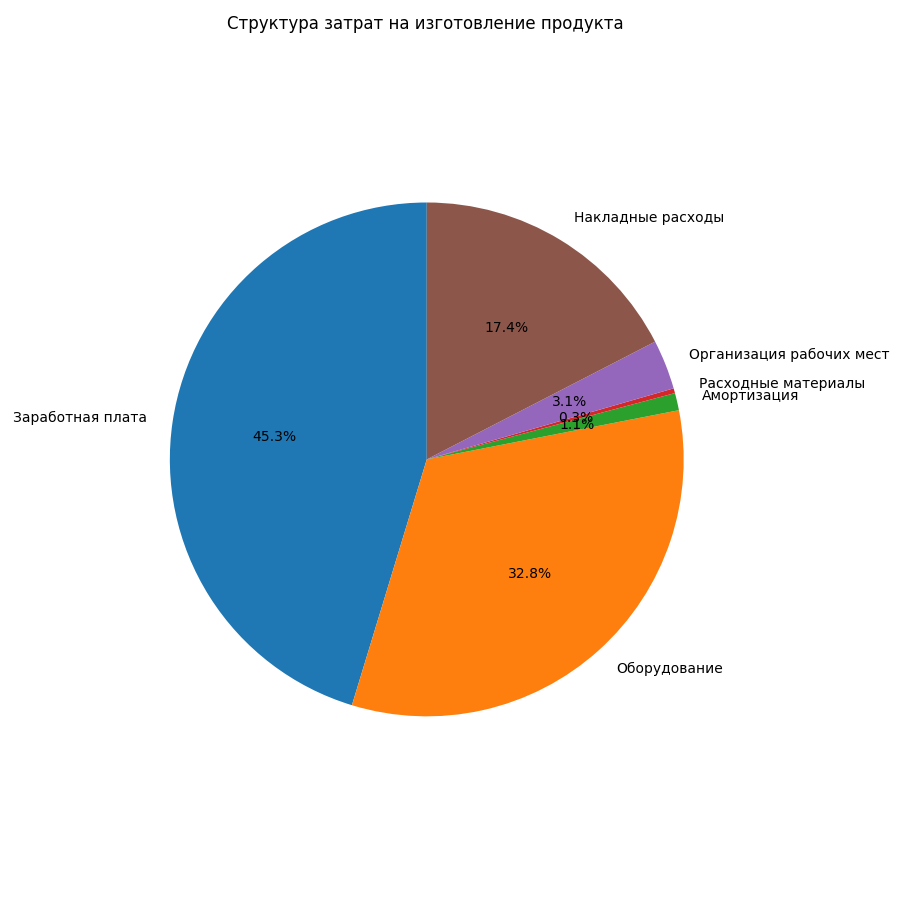
\includegraphics[width=0.6\textwidth]{inc/cost_dev.png}
\caption{Структура затрат на изготовление продукта}
\label{fig:cost_dev}
\end{figure}

\begin{figure}
\centering
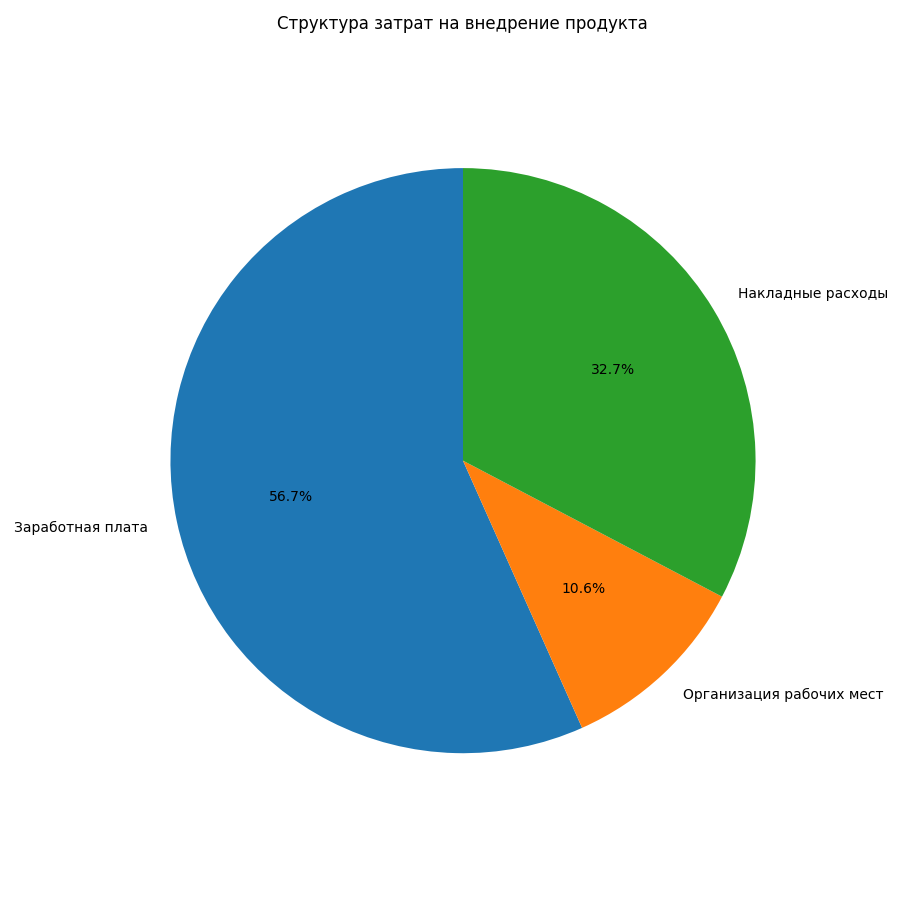
\includegraphics[width=0.6\textwidth]{inc/cost_impl.png}
\caption{Структура затрат на внедрение продукта}
\label{fig:cost_impl}
\end{figure}

